\chapter{Proverb 28}

\begin{figure}
  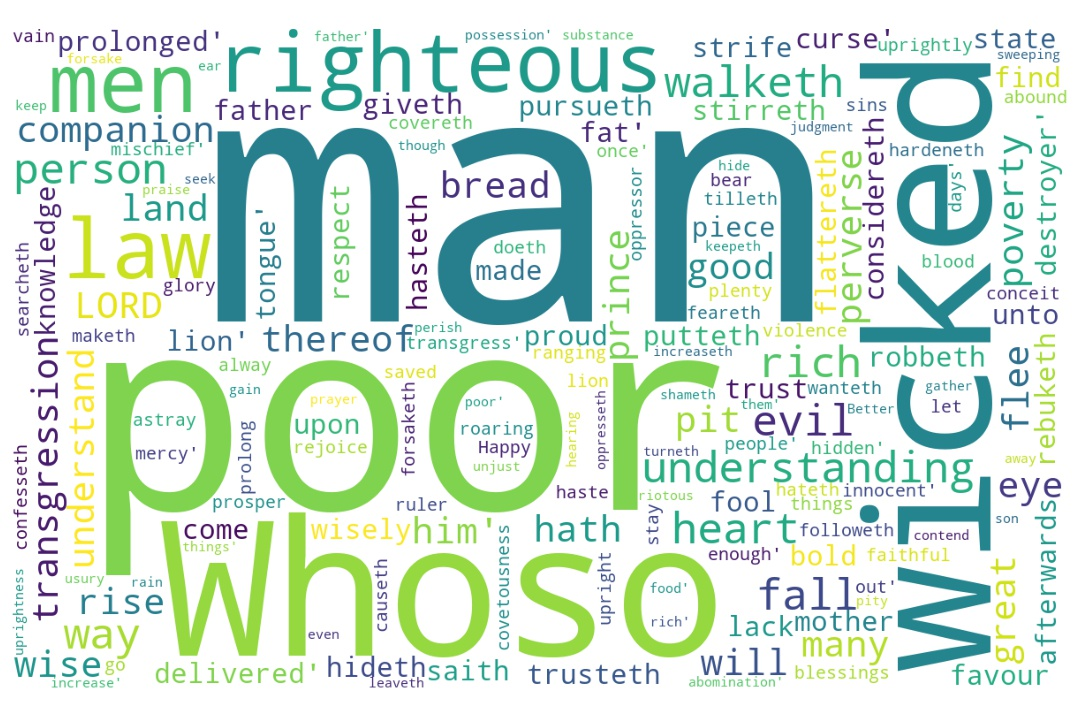
\includegraphics[width=\linewidth]{20OT-Proverbs/Proverb28-WordCloud.jpg}
  \caption{Proverb 28 Word Cloud}
  \label{fig:Proverb 28 word Cloud}
\end{figure}


\marginpar{\scriptsize \centering \fcolorbox{bone}{lime}{\textbf{RECOGNIZING THE WICKED}}\\ (Proverb 28:1--28)\begin{compactenum}[I.]
    \item \textbf{The Wicked Flee} They flee without being pursued, always afraid that their misdeeds are going to catch them. \index[scripture]{Proverbs!Pro 28:01}(Pro 28:1) 
    \item \textbf{The Wicked Forget} They forsake the law and are praised by other wicked for doing so. \index[scripture]{Proverbs!Pro 28:04}(Pro 28:4) 
    \item \textbf{The Wicked Forsakes his Father} \index[scripture]{Proverbs!Pro 28:07}(Pro 28:7)
    \item \textbf{The Wicked Fleece the Poor} \index[scripture]{Proverbs!Pro 28:08}(Pro 28:8) The wicked make their substance by usury and unjust gain, by cheating and dealing falsely.
    \item \textbf{The Wicked Fall into Their Own Pit} \index[scripture]{Proverbs!Pro 28:10}(Pro 28:10)
    \item \textbf{The Wicked are Foolish} \index[scripture]{Proverbs!Pro 28:16}(Pro 28:16)
    \item \textbf{The Wicked Follows his Own Heart} \index[scripture]{Proverbs!Pro 28:26}(Pro 28:26)
\end{compactenum}}

\marginpar{\scriptsize \centering \fcolorbox{bone}{yellow}{\textbf{THE WAYS OF THE WICKED}}\\ (Proverb 28) 
\begin{compactenum}[I.]
    \item \textbf{Perverts the Way of Right}  \index[scripture]{Proverbs!Pro 28:06}(Pro 28:6)
    \item \textbf{Oppresses the Poor} \index[scripture]{Proverbs!Pro 28:08}(Pro 28:8) 
    \item \textbf{Promotes only His Own Gain}  \index[scripture]{Proverbs!Pro 28:11} (Pro 28:11) 
    \item \textbf{Pretends to be Righteous}  \index[scripture]{Proverbs!Pro 28:13} (Pro 28:13) 
    \item \textbf{Pursues Wealth blindly} - It is blind ambition. \index[scripture]{Proverbs!Pro 28:22} (Pro 28:22)
    \item \textbf{Pilfers from his Parents}   \index[scripture]{Proverbs!Pro 28:24}(Pro 28:24)
    \item \textbf{Perish in Oblivion}  \index[scripture]{Proverbs!Pro 28:28}(Pro 28:28)
\end{compactenum}}

\marginpar{\scriptsize \centering \fcolorbox{bone}{black}{\textbf{\textcolor{white}{FOUR (FIVE) KINDS OF MEN}}}\\ (Proverb 28) 
\begin{compactenum}[I.]
    \item \textbf{Perverts the Way of Right}  \index[scripture]{Proverbs!Pro 28:06}(Pro 28:6)
    \item \textbf{Oppresses the Poor} \index[scripture]{Proverbs!Pro 28:08}(Pro 28:8) 
    \item \textbf{Promotes only His Own Gain}  \index[scripture]{Proverbs!Pro 28:11} (Pro 28:11) 
    \item \textbf{Pretends to be Righteous}  \index[scripture]{Proverbs!Pro 28:13} (Pro 28:13) 
    \item \textbf{Pursues Wealth blindly} - It is blind ambition. \index[scripture]{Proverbs!Pro 28:22} (Pro 28:22)
    \item \textbf{Pilfers from his Parents}   \index[scripture]{Proverbs!Pro 28:24}(Pro 28:24)
    \item \textbf{Perish in Oblivion}  \index[scripture]{Proverbs!Pro 28:28}(Pro 28:28)
\end{compactenum}}

\footnote{\textcolor[cmyk]{0.99998,1,0,0}{\hyperlink{TOC}{Return to end of Table of Contents.}}}\footnote{\href{https://www.audioverse.org/english/audiobibles/books/ENGKJV/O/Prov/1}{\textcolor[cmyk]{0.99998,1,0,0}{Proverbs Audio}}}\textcolor[cmyk]{0.99998,1,0,0}{The wicked flee when no man pursueth: but the righteous are bold as a lion.}
[2] \textcolor[cmyk]{0.99998,1,0,0}{For the \fcolorbox{bone}{MYGOLD}{transgression} of a land many \emph{are} the princes thereof: but by a man of \fcolorbox{bone}{MYGOLD}{understanding} \emph{and} knowledge the state \emph{thereof} shall be prolonged.}
[3] \textcolor[cmyk]{0.99998,1,0,0}{A poor man that oppresseth the poor \fcolorbox{bone}{bone}{\emph{is}} \emph{like} a sweeping rain which leaveth no food.}
[4] \textcolor[cmyk]{0.99998,1,0,0}{They that \fcolorbox{bone}{lime}{forsake} the law praise the wicked: but such as keep the law contend with them.}
[5] \textcolor[cmyk]{0.99998,1,0,0}{Evil men understand not judgment: but they that seek the LORD understand all \emph{things}.}
[6] \textcolor[cmyk]{0.99998,1,0,0}{Better \fcolorbox{bone}{bone}{\emph{is}} the poor that walketh in his uprightness, than \emph{he} \emph{that} \fcolorbox{bone}{bone}{\emph{is}} \fcolorbox{bone}{lime}{perverse} \emph{in} \emph{his} ways, though he \emph{be} rich.}
[7] \textcolor[cmyk]{0.99998,1,0,0}{Whoso keepeth the law \fcolorbox{bone}{bone}{\emph{is}} a wise son: but he that is a companion of riotous \emph{men} shameth his father.}
[8] \textcolor[cmyk]{0.99998,1,0,0}{He that by usury and \fcolorbox{bone}{lime}{unjust gain} increaseth his substance, he shall gather it for him that will pity the poor.}
[9] \textcolor[cmyk]{0.99998,1,0,0}{He that \fcolorbox{bone}{lime}{turneth} away his ear from hearing the law, even his prayer \emph{shall} \emph{be} abomination.}
[10] \textcolor[cmyk]{0.99998,1,0,0}{Whoso causeth the righteous to go astray in an evil way, he shall fall himself into his own pit: but the upright shall have good \emph{things} in possession.}
[11] \textcolor[cmyk]{0.99998,1,0,0}{The rich man \fcolorbox{bone}{bone}{\emph{is}} wise in his own \fcolorbox{bone}{lime}{conceit}; but the poor that hath \fcolorbox{bone}{MYGOLD}{understanding} searcheth him out.}
[12] \textcolor[cmyk]{0.99998,1,0,0}{When righteous \emph{men} do rejoice, \emph{there} \fcolorbox{bone}{bone}{\emph{is}} great glory: but when the wicked rise, a man is hidden.}
[13] \textcolor[cmyk]{0.99998,1,0,0}{He that covereth his sins shall not prosper: but whoso confesseth and forsaketh \emph{them} shall have mercy.}
[14] \textcolor[cmyk]{0.99998,1,0,0}{Happy \fcolorbox{bone}{bone}{\emph{is}} the man that feareth alway: but he that hardeneth his heart shall fall into mischief.}
[15] \textcolor[cmyk]{0.99998,1,0,0}{\emph{As} a roaring lion, and a ranging bear; \emph{so} \fcolorbox{bone}{bone}{\emph{is}} a wicked ruler over the poor people.}
[16] \textcolor[cmyk]{0.99998,1,0,0}{The prince that wanteth \fcolorbox{bone}{MYGOLD}{understanding} \fcolorbox{bone}{bone}{\emph{is}} also a great oppressor: \emph{but} he that hateth covetousness shall prolong \emph{his} days.}
[17] \textcolor[cmyk]{0.99998,1,0,0}{A man that doeth violence to the blood of \emph{any} person shall flee to the pit; let no man stay him.}
[18] \textcolor[cmyk]{0.99998,1,0,0}{Whoso walketh uprightly shall be saved: but \emph{he} \emph{that} \fcolorbox{bone}{bone}{\emph{is}} perverse \emph{in} \emph{his} ways shall fall at once.}
[19] \textcolor[cmyk]{0.99998,1,0,0}{He that tilleth his land shall have plenty of bread: but he that followeth after vain \emph{persons} shall have poverty enough.}\footnote{\textbf{Psalm 26:4} -  have not sat with vain persons, neither will I go in with dissemblers.}\footnote{\textbf{Proverb 12:11} - He that tilleth his land shall be satisfied with bread: but he that followeth vain persons is void of understanding.}
[20] \textcolor[cmyk]{0.99998,1,0,0}{A faithful man shall abound with blessings: but he that maketh haste to be rich shall not be innocent.}
[21] \textcolor[cmyk]{0.99998,1,0,0}{To have respect of persons \fcolorbox{bone}{bone}{\emph{is}} not good: for  a piece of bread \emph{that} man will transgress.}
[22] \textcolor[cmyk]{0.99998,1,0,0}{He that hasteth to be rich \emph{hath} an evil eye, and considereth not that poverty shall come upon him.}
[23] \textcolor[cmyk]{0.99998,1,0,0}{He that rebuketh a man afterwards shall find more favour than he that flattereth with the tongue.}
[24] \textcolor[cmyk]{0.99998,1,0,0}{Whoso robbeth his father or his mother, and saith, \emph{It} \fcolorbox{bone}{bone}{\emph{is}} no \fcolorbox{bone}{MYGOLD}{transgression}; the same \fcolorbox{bone}{bone}{\emph{is}} the companion of a destroyer.}\footnote{\textbf{Mark 7:9-13} - And he said unto them, Full well ye reject the commandment of God, that ye may keep your own tradition. [10] For Moses said, Honour thy father and thy mother; and, Whoso curseth father or mother, let him die the death: [11] But ye say, If a man shall say to his father or mother, It is Corban, that is to say, a gift, by whatsoever thou mightest be profited by me; he shall be free. [12] And ye suffer him no more to do ought for his father or his mother; [13] Making the word of God of none effect through your tradition, which ye have delivered: and many such like things do ye.}
[25] \textcolor[cmyk]{0.99998,1,0,0}{He that is of a proud heart stirreth up strife: but he that putteth his trust in the LORD shall be made fat.}
[26] \textcolor[cmyk]{0.99998,1,0,0}{He that trusteth in his own heart is a fool: but whoso walketh wisely, he shall be delivered.}\footnote{\textbf{Jeremiah 17:9} - The heart is deceitful above all things, and desperately wicked: who can know it? [10] I the LORD search the heart, I try the reins, even to give every man according to his ways, and according to the fruit of his doings.}
[27] \textcolor[cmyk]{0.99998,1,0,0}{He that giveth unto the poor shall not lack: but he that hideth his eyes shall have many a curse.}
[28] \textcolor[cmyk]{0.99998,1,0,0}{When the \fcolorbox{bone}{lime}{wicked} rise, men hide themselves: but when they perish, the righteous increase.}



